\documentclass[12pt,a4paper,oneside]{article}
\usepackage[utf8]{vietnam}
\usepackage{amsmath}
\usepackage{amsfonts}
\usepackage{amssymb}
\usepackage{graphicx}
\usepackage[left=2cm,right=2cm,top=2cm,bottom=2cm]{geometry}
\usepackage{array}
\usepackage{fancyhdr}
\pagestyle{fancy}
\renewcommand\thesection{\Roman{section}.}
\renewcommand\thesubsection{\arabic{subsection}.}
\fancyhf{}
\rhead{\textbf{Final Project}}
\lhead{Hoàng Quốc Bảo - 20194484}
\rfoot{Trang \thepage}
\usepackage{listings}
\usepackage{tcolorbox}
\usepackage{color} % tô màu cho code
\definecolor{dkgreen}{rgb}{0,0.6,0}
\definecolor{gray}{rgb}{0.5,0.5,0.5}
\definecolor{code}{rgb}{0.8,0.8,0.8}
\definecolor{mauve}{rgb}{0.58,0,0.82}
\lstset{frame=tb,
  language=[x86masm]Assembler,
  aboveskip=3mm,
  belowskip=3mm,
  showstringspaces=false,
  columns=flexible,
  basicstyle={\small\ttfamily},
  backgroundcolor=\color{gray!20!white},
  numbers=none,
  breaklines=true,
  breakatwhitespace=true,
  tabsize=3
}

\begin{document}
\begin{center}
\begin{large}
\thispagestyle{empty}
\textbf{ĐẠI HỌC BÁCH KHOA HÀ NỘI}\\
\textbf{TRƯỜNG CÔNG NGHỆ THÔNG TIN VÀ TRUYỀN THÔNG}\\[0.5in]
\end{large}

\includegraphics[scale=0.2]{image/hust}\\[0.5in]
\textbf{{\Large BÁO CÁO PROJECT CUỐI KÌ MÔN KIẾN TRÚC MÁY TÍNH}}\\[0.25in]
\textbf{Giảng viên hướng dẫn: } Nguyễn Văn Hiên\\[0.5in]
\begin{flushleft}
Nhóm 2:\\
\qquad Hoàng Quốc Bảo - 20194484\\
\qquad Vũ Minh Hải - 20194550
\end{flushleft}
\end{center}
\pagebreak
\section*{Exercise 3:}
\textbf{Đề bài: \\}
Chương trình sau sẽ đo tốc độ gõ bàn phím và hiển thị kết quả bằng 2 đèn led 7 đoạn. Nguyên tắc:
\begin{itemize}
\item Cho một đoạn văn bản mẫu, cố định sẵn trong mã nguồn. Ví dụ “bo mon ky thuat may tinh”
\item Sử dụng bộ định thời Timer (trong bộ giả lập Digi Lab Sim) để tạo ra khoảng thời gian để đo. Đây là thời 
gian giữa 2 lần ngắt, chu kì ngắt.
\item Trong thời khoảng đó, người dùng nhập các kí tự từ bàn phím. Ví dụ nhập “bo mOn ky 5huat may tinh”.
\end{itemize}
Chương trình cần phải đếm số kí tự đúng (trong ví dụ trên thì người dùng gõ sai chữ O và 5) mà người dùng đã gõ và hiển thị lên các đèn led\\\\
\textbf{Lưu đồ thuật toán:}
\begin{center}
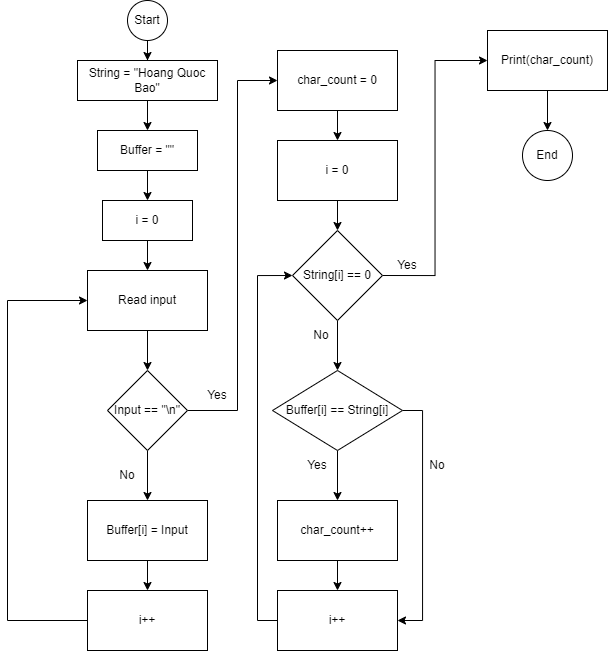
\includegraphics[scale=0.7]{image/flowchartb3}
\end{center}
\pagebreak
\textbf{Mã nguồn:}
\begin{lstlisting}
# MMIO Simulator
.eqv KEY_CODE		0xFFFF0004
.eqv KEY_READY		0xFFFF0000
.eqv DISPLAY_CODE 	0xFFFF000C 	# ASCII code to show, 1 byte
.eqv DISPLAY_READY 	0xFFFF0008 	# =1 if the display has already to do
 					# Auto clear after sw
.eqv COUNTER            0xFFFF0013 	# Time counter 			
# Led 7 doan			
.eqv SEVENSEG_RIGHT 	0xFFFF0010 	# Dia chi cua den led 7 doan phai
.eqv SEVENSEG_LEFT	0xFFFF0011 	# Dia chi cua den led 7 doan trai

.data
	string: .asciiz "Hoang Quoc Bao"
	buffer: .space 100
	count_char: .asciiz "\nSo ki tu dung: "
	toc_do: .asciiz "\nToc do go phim: "
	don_vi: .asciiz "chu ki/ki tu"
	
.text
	li $t0, 1
	li $a0, COUNTER 	
	sb $t0, 0($a0)			# Gan bit COUNTER khac 0 de kich hoat ngat
	li $t0, 0			# i = 0
	li $s0, 0			# So chu ki ngat
	li $t8, 0			# $t8 = 0 : chua dem, = 1 : bat dau dem
	
in_string_mau:
WaitForDis:
	lw $t2, DISPLAY_READY
	beq $t2, $zero, WaitForDis	# Neu $t2 = 0 thi tiep tuc cho
					# display san sang
	nop
	lb $t1, string($t0)		# $s1 = string[i]
	beq $t1, '\0', doc_ban_phim	# Neu string[i] == NULL thi break
	sw $t1, DISPLAY_CODE		# Hien thi string[i] ra man hinh
	add $t0, $t0, 1			# i++
	j in_string_mau			# Tiep tuc in cho den het string
	
doc_ban_phim:
	li $t0, 0			# i = 0
	
WaitForKey:
	lw $k1, KEY_READY
	beq $k1, $zero, WaitForKey	# Neu $k1 = 0 thi tiep tuc cho
					# keyboard san sang
	nop
	li $t8, 1			# $t8 = 1 : bat dau dem cac chu ki ngat
	lw $k0, KEY_CODE		# Doc ki tu tu ban phim
	beq $k0, 10, exit		# Ket thuc go neu nguoi dung nhan nut Enter
	
	sb $k0, buffer($t0)		# Luu lai phim vua go
	
	add $t0, $t0, 1			# i++
	j WaitForKey			# Tiep tuc doc ki tu tu ban phim
	
exit:
	li $v0, 4
	la $a0, buffer
	syscall				# In xau da nhap vao tu ban phim
	
	li $v0, 4
	la $a0, toc_do
	syscall				# In ra man hinh: "Toc do go phim: "
	
	mtc1 $t0, $f1			# Convert $t0(integer) -> $f1(float): so ki tu da nhap
	mtc1 $s0, $f2			# Convert $s0(integer) -> $f2(float): so chu ki ngat
	div.s $f12, $f2, $f1		# Toc do go phim = So chu ki ngat / So ki tu da nhap
	# div $a0, $s0, $t0		
	li $v0, 2
	syscall
	
	# li $v0, 1
	# syscall				# In ra toc do go phim
	
	li $v0, 4
	la $a0, don_vi			# In ra "chu ki/ki tu"
	syscall
	
Char_counting:
	li $s4, 0			# $s4 = so ki tu go chinh xac
	li $t0, 0			# i = 0
strcmp:
	lb $t1, string($t0)		# $t1 = string[i]
	lb $t2, buffer($t0)		# $t2 = string[i]
	beq $t1, $zero, mess 		# if string[i] == NULL then break
	
	bne $t1, $t2, next_char		# if string[i] == buffer[i] then
	add $s4, $s4, 1			# dung++
next_char:
	add $t0, $t0, 1			# i++
	j strcmp			# Tiep tuc so sanh cho den het chuoi
	
mess:
	li $v0, 4
	la $a0, count_char
	syscall				# In ra man hinh: "So ki tu dung: "
	
	add $a0, $zero, $s4		
	li $v0, 1
	syscall				# In so ki tu go dung
	
	
	li $t4, 10
	div $s4, $t4			# Chia so ki tu go dung cho 10

	mflo $t0			# $t0 = $s4 / $t4 (hang chuc)
	jal SET_DATA_FOR_7SEG
	add $a1, $zero, $a0		# Led ben trai = hang chuc
	
	mfhi $t0			# $t0 = phep du $s4 / $t4 (hang don vi)
	jal SET_DATA_FOR_7SEG
	
	jal SHOW_7SEG_RIGHT		# Hien thi hang don vi o led ben phai
	jal SHOW_7SEG_LEFT		# Hien thi hang chuc o led ben trai
		
	li $v0, 10
	syscall				# Goi thu tuc ket thuc chuong trinh
	
SHOW_7SEG_RIGHT:
# input: $a0
	sb $a0, SEVENSEG_RIGHT	
	jr $ra

SHOW_7SEG_LEFT:
# input: $a1
	sb $a1, SEVENSEG_LEFT
	jr $ra

SET_DATA_FOR_7SEG:
# input: $t0
	beq $t0, 0, set0
	nop
	beq $t0, 1, set1
	nop
	beq $t0, 2, set2
	nop
	beq $t0, 3, set3
	nop
	beq $t0, 4, set4
	nop
	beq $t0, 5, set5
	nop
	beq $t0, 6, set6
	nop
	beq $t0, 7, set7
	nop
	beq $t0, 8, set8
	nop
	beq $t0, 9, set9
	nop
set0:	li $a0, 0x3f
	j done_set
	nop
set1: 	li $a0, 0x06
	j done_set
	nop 
set2: 	li $a0, 0x5b
	j done_set
	nop
set3: 	li $a0, 0x4f
	j done_set
	nop
set4: 	li $a0, 0x66
	j done_set
	nop
set5: 	li $a0, 0x6d
	j done_set
	nop
set6: 	li $a0, 0x7d
	j done_set
	nop
set7: 	li $a0, 0x07
	j done_set
	nop
set8: 	li $a0, 0x7f
	j done_set
	nop
set9: 	li $a0, 0x6f
	j done_set
	nop
done_set:
	jr $ra
	
# Xu ly ngat

.ktext 0x80000180
IntSR:
	add $t9, $zero, $at		# Luu lai gia tri thanh ghi $at
	mfc0 $v0, $13			# Kiem tra ma nguyen nhan ngat
	bne $v0, 1024, exit		# Ma ngat 1024, bo qua ma ngat do Counter cua Digit Lab Sim
					# Neu la ma ngat khac => loi => ket thuc chuong trinh
	add $s0, $s0, $t8		# Tang bien dem so chu ki ngat
					# => Bien dem $s0 chi tang khi $t8 = 1 (khi bat dau go)
	move $at, $t9			# Khoi phuc thanh ghi $at
return:
	eret				# Quay lai vi tri ngat
\end{lstlisting}
\pagebreak
\textbf{Giải thích:}
\begin{itemize}
\item Đầu tiên, gán tên và địa chỉ cho các thanh ghi tường ứng
\begin{center}
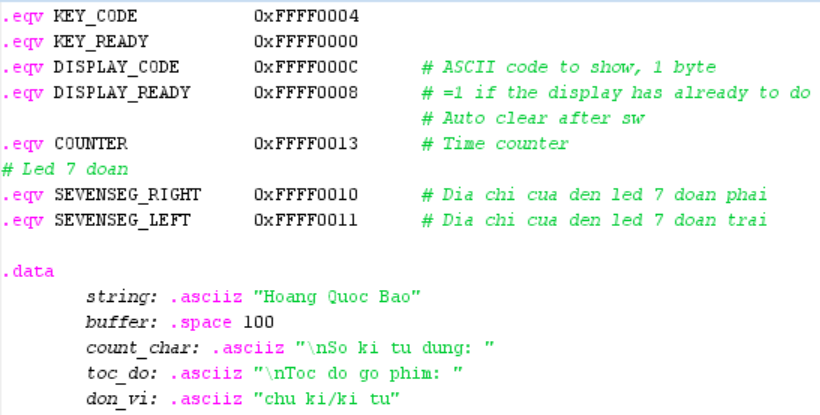
\includegraphics[scale=1]{image/b31}
\end{center}
\item Khởi tạo các biến
\begin{center}
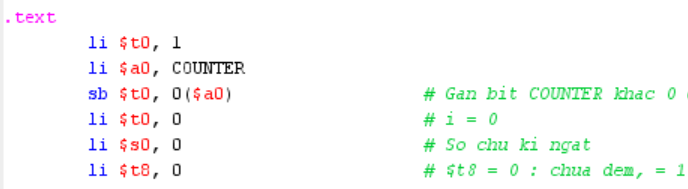
\includegraphics[scale=1]{image/b32}
\end{center}
Trong đó:
\begin{itemize}
\item Thanh ghi \$t0 đếm số kí tự đã được nhập vào từ bàn phím.
\item Thanh ghi \$s0 đếm số chu kì ngắt.
\item Thanh ghi \$t8 quy định việc đếm chu kì ngắt bắt đầu hay chưa. (Đếm bắt đầu khi keyboard được kết nối với MIPS)
\end{itemize}
\item In xâu kí tự mẫu ra Display
\begin{center}
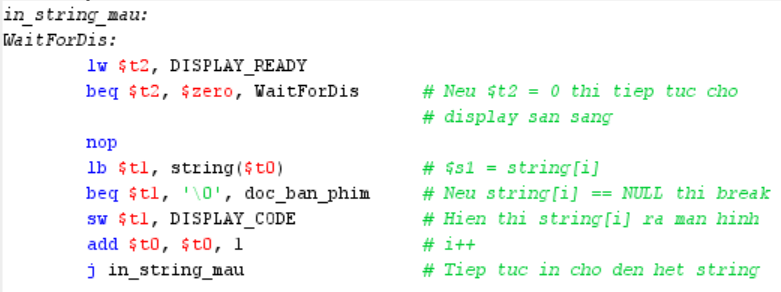
\includegraphics[scale=1]{image/b33}
\end{center}
\pagebreak
Kết quả thực hiện:
\begin{center}
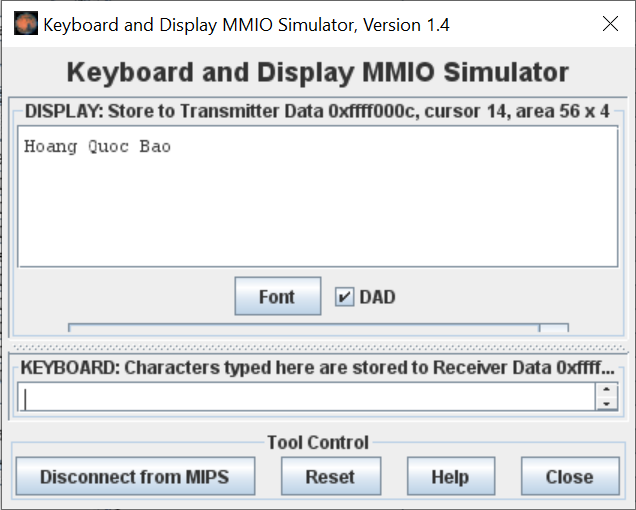
\includegraphics[scale=1]{image/b34}
\end{center}
\item Đọc xâu từ bàn phím
\begin{center}
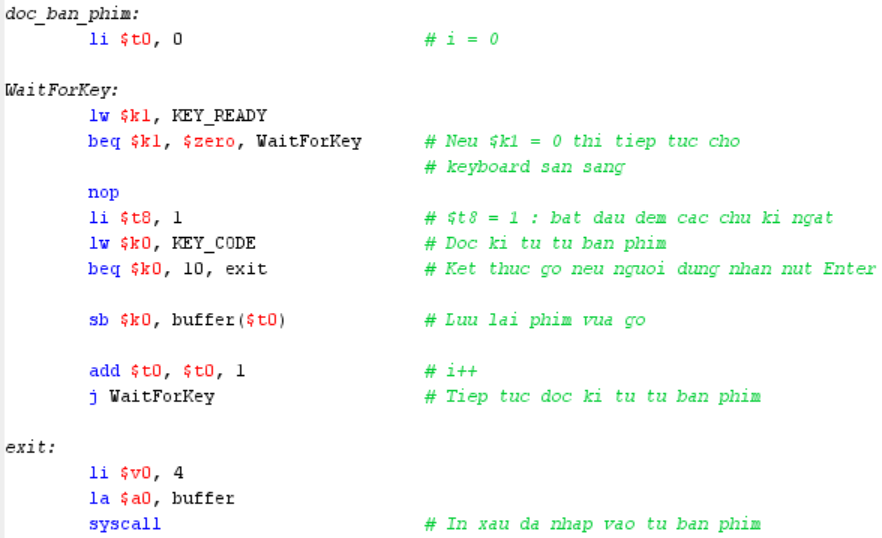
\includegraphics[scale=1]{image/b35}
\end{center}
Chương trình thực hiện đọc xâu kí tự từ bàn phím. Việc đọc kết thúc khi người dùng nhập vào phím \textit{Enter}. Sau khi đọc xong, in ra màn hình xâu đã đọc được.\\\\\\\\\\\\

Nhập vào xâu:
\begin{center}
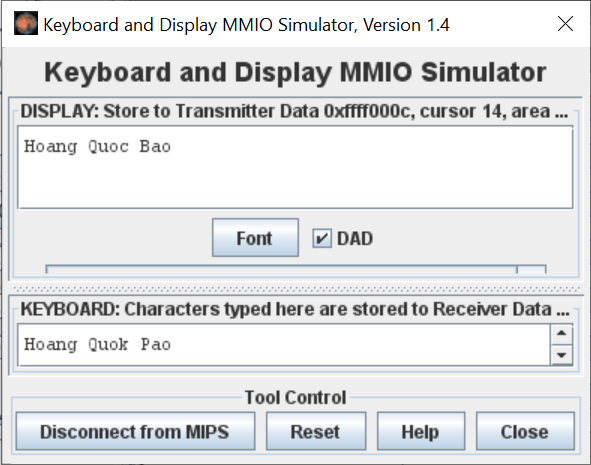
\includegraphics[scale=1]{image/b36}
\end{center}
Kết quả thực hiện:
\begin{center}
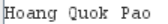
\includegraphics[scale=1]{image/b37}
\end{center}
\item In ra console tốc độ gõ phím
\begin{center}
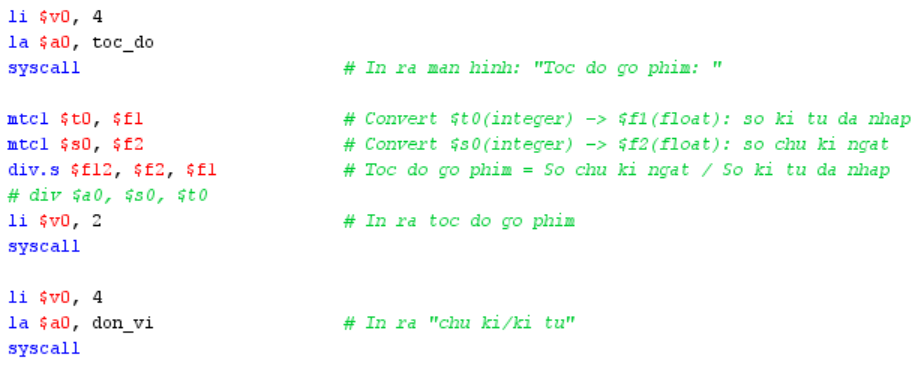
\includegraphics[scale=1]{image/b38}
\end{center}
Đoạn chương trình in ra màn hình tốc độ gõ phím. Trong đó \textit{Tốc độ gõ phím = Số chu kì ngắt / Số kí tự đã nhập}. (Đơn vị: Chu kì / kí tự). \\Được tính chính xác đến chữ số thập phân.
\pagebreak
\item Tính số kí tự gõ chính xác
\begin{center}
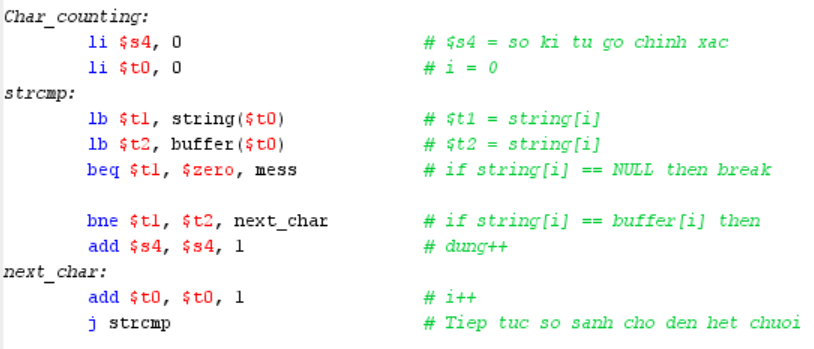
\includegraphics[scale=1]{image/b40}
\end{center}
Chương trình thực hiện so sánh hai xâu \textit{String} và \textit{Buffer} bằng cách so sánh từng phần từ, nếu 2 phần tử giống nhau thì tăng biến đếm \$s4 lên 1 đơn vị. Tiếp tục lặp lại cho đến hết dãy.
\item In ra số kí tự chính xác trên console
\begin{center}
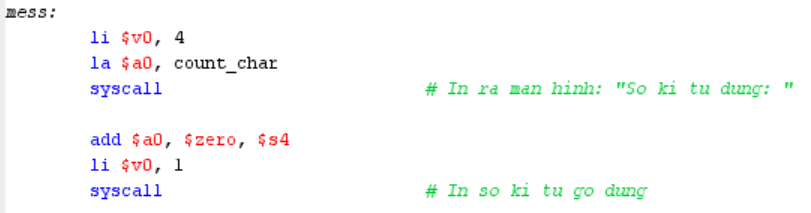
\includegraphics[scale=1]{image/b41}
\end{center}
\item In ra số kí tự chính xác trên Led 7 đoạn
\begin{center}
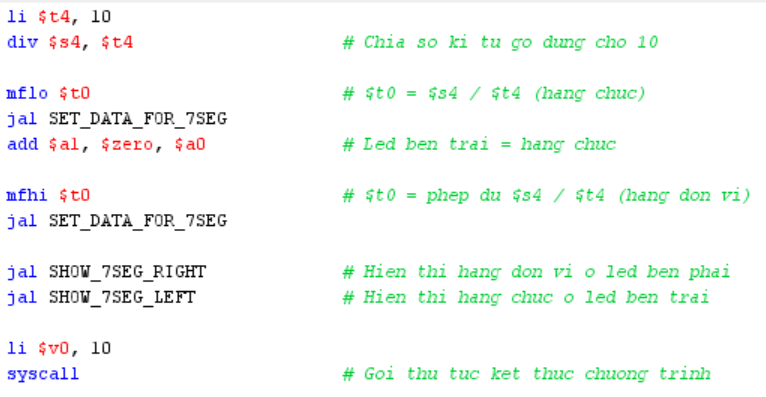
\includegraphics[scale=1]{image/b42}
\end{center}
Chương trình sẽ thực hiện lấy giá trị nhanh ghi \$s4 (đếm số kí tự gõ chính xác) chia cho 10. Giá trị thương sẽ được hiển thị lên  Led 7 đoạn bên trái, còn số dư sẽ được hiển thị lên Led 7 đoạn bên phải.
\pagebreak
\item Kết quả thực hiện:
\begin{center}
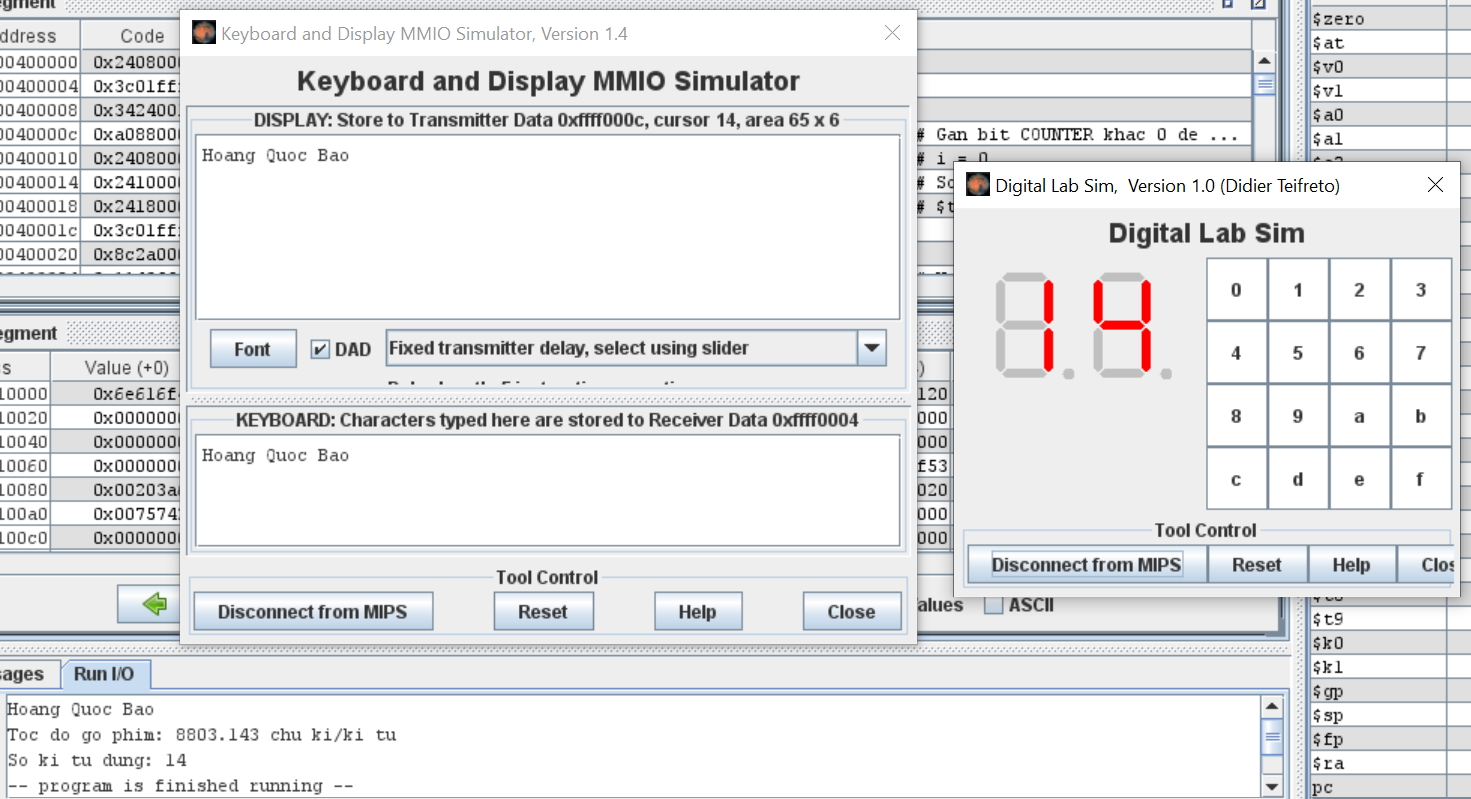
\includegraphics[scale=0.6]{image/b43}
\end{center}
\end{itemize}


\end{document}